\documentclass{scrbook}
\usepackage{tcolorbox}
\usepackage{hyperref} %for better referencing
\title{Fundamental Theorum of Calculus and its problematic discontinuities}
\author{mathGhost}

%%PAGE GEOMETRY and PAGE SETUP, as in header/footer/footnote
%%-----------------------------------------------------------------------
%%-----------------------------------------------------------------------
\usepackage[a4paper, bindingoffset=6mm,
headheight=15.2pt % use geometry to change the head height
]{geometry}

\usepackage[headsepline,automark,autooneside=false]{scrlayer-scrpage}% sets pagestyle scrheadings automatically
\renewcommand*\chaptermarkformat{}% remove chapter number from header entry
\renewcommand*\sectionmarkformat{}% remove section number from header entry

\clearpairofpagestyles% before setting the new contents of header and footer
\cfoot*{\pagemark}
\ihead{\rightmark}
\ohead{\leftmark}
\addtokomafont{pageheadfoot}{\upshape}

% page style empty in TOC, LOF, LOT and all other lists under controll of  package tocbasic
%\AfterTOCHead{\thispagestyle{empty}\pagestyle{empty}}
%\AfterStartingTOC{\thispagestyle{empty}}

\usepackage{blindtext}% only for dummy text

\usepackage[bottom]{footmisc}                    %createsfootnotes
%%-----------------------------------------------------------------------
%%-----------------------------------------------------------------------

%%MATHEMATICAL PACKAGES
%%-----------------------------------------------------------------------
%%-----------------------------------------------------------------------
\usepackage{physics,amsthm, amsmath,esint}
\usepackage{amssymb}
\usepackage{amsfonts}
\usepackage{tcolorbox}
%%-----------------------------------------------------------------------
%%-----------------------------------------------------------------------

%%GRAPHICS PACKAGES
%%----------------------------------------------------------------------
%%----------------------------------------------------------------------
\usepackage{graphicx}               %needed for the insertion of graphics, remove draft for final script.
\graphicspath{{./images/}}            %needed for choosing the image path
\usepackage{caption}             %needed for captioning of a single image
\captionsetup{justification = raggedright, singlelinecheck = false} %forces left-alignment of captions
\usepackage{subcaption}         %needed for allowing 'sub'-captioning of multiple-images
\setcapindent{2cm}                   %indents the caption borders to zero
\usepackage{float}	                         %allows using [H] for images
\usepackage[font={small}]{caption} %image captions in different fonts
%\usepackage{float}
%\floatstyle{boxed} 
%\restylefloat{figure}          %defines a border for all the float images
%%-----------------------------------------------------------------------
%%-----------------------------------------------------------------------



%%PACKAGE FOR APPENDICES
%%-----------------------------------------------------------------------
%%-----------------------------------------------------------------------
\usepackage[toc,page]{appendix}
%%-----------------------------------------------------------------------
%%-----------------------------------------------------------------------

%%PACKAGE FOR CODE INDENTATION
\usepackage{listings}
\usepackage{color}

\definecolor{dkgreen}{rgb}{0,0.6,0}
\definecolor{gray}{rgb}{0.5,0.5,0.5}
\definecolor{mauve}{rgb}{0.58,0,0.82}

\lstset{frame=tb,
	language=Python,
	aboveskip=3mm,
	belowskip=3mm,
	showstringspaces=false,
	columns=flexible,
	basicstyle={\small\ttfamily},
	numbers=none,
	numberstyle=\tiny\color{gray},
	keywordstyle=\color{blue},
	commentstyle=\color{dkgreen},
	stringstyle=\color{mauve},
	breaklines=true,
	breakatwhitespace=true,
	tabsize=3
}
\begin{document}
	\maketitle
	\tableofcontents
	\chapter{Definite Integrals with Substitutions}
\label{chap:1}
Focussing on the definite integral, $I =\int_{-\infty}^{+\infty}A\,\mathrm{d}x$. It brings up contradictory results as shown in proof.\ref{P1}
\begin{proof}[Proof 1]\label{P1}
	If $$A > 0, \implies I = \int_{-\infty}^{+\infty}A\,\mathrm{d}x \to \infty$$
	but if we break up the integral as in,
	$$I = \int_{-\infty}^{+\infty}A\,\mathrm{d}x = \int_{-\infty}^{-1}A\,\mathrm{d}x + \int_{-1}^{+1}A\,\mathrm{d}x + \int_{+1}^{+\infty}A\,\mathrm{d}x$$
	$$\implies I = 2A + \int_{-\infty}^{-1}A\,\mathrm{d}x + \int_{+1}^{+\infty}A\,\mathrm{d}x$$
	Substituting $$x = \frac{1}{y}\, \implies \mathrm{d}x = -\frac{1}{y^2} \mathrm{d}y$$
	We get;
	$$I = 2A +A\int_{-1}^{0} \frac{1}{y^2}\,\mathrm{d}y +A\int_{0}^{1} \frac{1}{y^2}\,\mathrm{d}y = 2A + A\int_{-1}^{1}\frac{1}{y^2}\,\mathrm{d}y$$
	$$\implies I = 2A + A(\frac{1}{y}\bigg\rvert_{1}^{-1}) = 0 $$
\end{proof}
The problem seems to be with the integral $I' = \int_{-1}^{+1}\frac{1}{y^2}\,\mathrm{d}y$. But, if we break it up into two integrals as shown in proof.\ref{P2}, Then the entire integral diverges as expected.
\begin{proof}[Proof 2]\label{P2}
	$$I' = \int_{-1}^{+1}\frac{1}{y^2}\,\mathrm{d}y$$
	\begin{align*}
		& = \int_{-1}^{0^-}\frac{1}{y^2}\,\mathrm{d}y + \int_{0^+}^{+1}\frac{1}{y^2}\,\mathrm{d}y \\
		& = -\bigg(\, \frac{1}{y}\bigg\rvert_{-1}^{0^-} + \frac{1}{y}\bigg\rvert_{0^+}^{+1}\,\bigg)\\
		& \to +\infty &&
	\end{align*}
\end{proof}
It is also to be noted that the divergence of the integral $I'$ is expected because as can be seen from proof.\ref{P1}, $I = 2A + I'$ and $I \to \infty$, hence it has to logically follow that $I' \to \infty$. But, it is noteworthy looking at the graph of fig.\ref{F1a} which shows the increase in the integral area $I'$ around the point $x=0$.
\begin{figure}[h]
	\centering
	\begin{subfigure}[t]{0.49\textwidth}
		\centering
		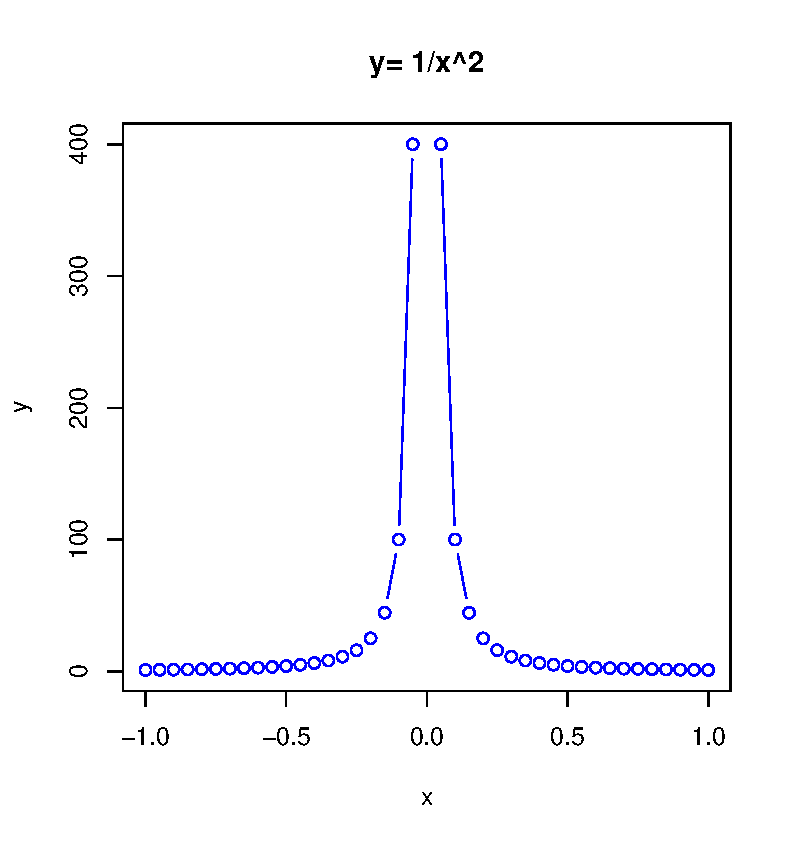
\includegraphics[width=\linewidth]{Plot1a.pdf}
		\phantomsubcaption
		\label{F1a}
	\end{subfigure}
	\hfill
	\begin{subfigure}[t]{0.49\textwidth}
		\centering
		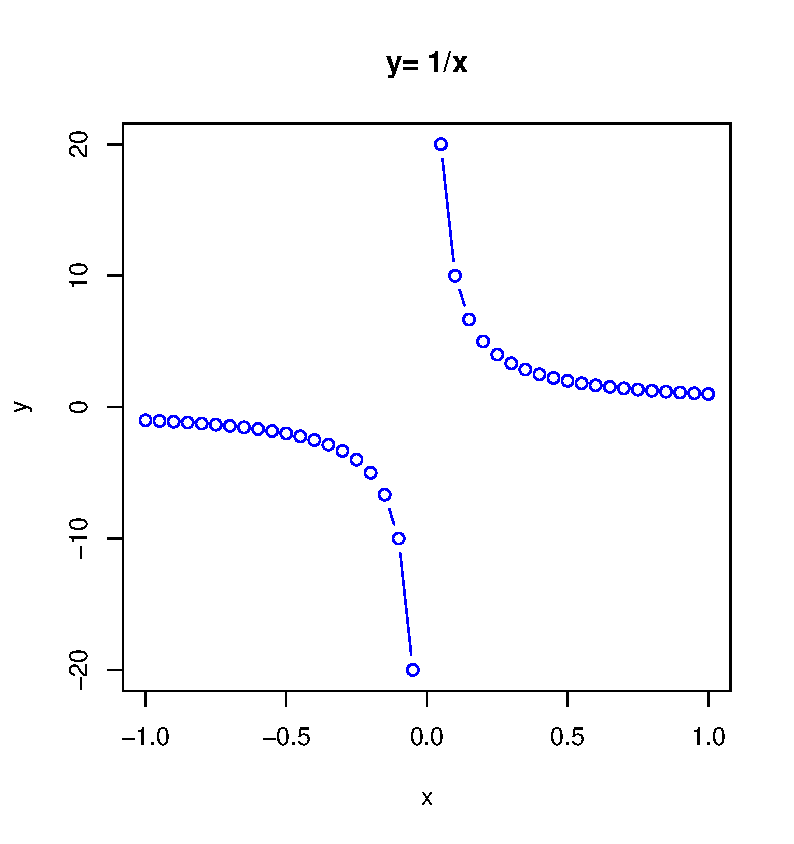
\includegraphics[width=\linewidth]{Plot1b.pdf}
		\phantomsubcaption
		\label{F1b}
	\end{subfigure}
	\caption{(a)Plot of $y=1/x^2$ generated using R. (b)Plot of $y = 1/x$ generated using R.}\label{F1}
\end{figure}
It is noteworthy to see that since $\lim_{x \to 0^-}1/x^2 = \lim_{x \to 0^+}1/x^2$, hence there is no discontinuity at the point $x = 0$, but it is important to note that the antiderivative $1/x$ is discontinuous at $x=0$ as seen in fig.\ref{F1b}, and also the function $1/x^2$ is not differentiable at the point $x=0$ since the derivative of $1/x^2$ is $-2/x^3$ and the derivative is not continuous at $x=0$, that is, the $\lim_{x \to 0^-} 2/x^3 \neq \lim_{x \to 0^+}2/x^3$.\\

To answer the question as to why the discontinuity of the antiderivate matters for an integral taken over the interval containing the point in question, we need to look closely at the \textit{fundamental theorum of calculus} talked about in \autoref{chap:2}.
	\chapter{Fundamental Theorum of Calculus}
\label{chap:2}
\begin{tcolorbox}
	The fundamental theorum of calculus states that if $I = \int_{a}^{b}f(x)\,\mathrm{d}x$ and if $g(x)$ is the antiderivative of $f(x)$ such that $f(x) = \mathrm{d}g(x)/\mathrm{d}x$, then $I = \int_{a}^{b}f(x)\,\mathrm{d}x = g(b)-g(a)$.
\end{tcolorbox}

We use the fundamental theorum of calculus for everyday integration, since using the riemann summation would otherwise be too cumbersome.\\

\begin{tcolorbox}
	The riemann summation is defined with respect to the area of a curve and is the definition of the integration operation in its most native form. Hence, it is defined as $$I = \int_{a}^{b}f(x)\,\mathrm{d}x = \lim_{\Delta x \to 0} \sum_{n=0}^{\frac{b-a}{\Delta x} - 1}f(a + n\Delta x)\Delta x$$
\end{tcolorbox}
The definition of the riemann summation converges to the fundamental theorum of calculus under certain approximations. This shown in proof.\ref{P3}.

\begin{proof}[Proof 3]\label{P3}
Iff
	\begin{equation}
	I = \int_{a}^{b}f(x)\,\mathrm{d}x = \lim_{\Delta x \to 0}\sum_{n=0}^{\frac{b-a}{\Delta x}-1}f(a + n \Delta x)\Delta x \label{eqn: 2.1}
	\end{equation}
and iff, $g(x)$ is the antiderivative of $f(x)$, then
\begin{equation}
	f(x) = \frac{\mathrm{d}g(x)}{\mathrm{d}x} = \lim_{\Delta x \to 0} \frac{g(x + \Delta x) - g(x)}{\Delta x} \label{eqn: 2.2}
\end{equation}
From \eqref{eqn: 2.2} we can write \eqref{eqn: 2.3}
\begin{equation}
	\lim_{\Delta x \to 0}f(x)\Delta x = \lim_{\Delta x \to 0} g(x + \Delta x) - g(x) \label{eqn: 2.3}
\end{equation}
It follows from \eqref{eqn: 2.3} that...
\begin{align*}
	I = \lim_{\Delta x \to 0}\sum_{n=0}^{\frac{b-a}{\Delta x}-1}f(a + n\Delta x) \Delta x &= \lim_{\Delta x \to 0}\sum_{n=0}^{\frac{b-a}{\Delta x}-1}g(a + (n+1)\Delta x) - g(a + n\Delta x)\\
	&= g(a + \Delta x) - g(a)\\
	&+ g(a + 2\Delta x) - g(a + \Delta x)\\
	&+ g(a + 3\Delta x) - g(a + 2\Delta x)\\
	&+ ....\\
	&+ ....\\
	&+ g(b) - g(b - \Delta x)&&
\end{align*}
Following the summation sequence shown above, we are left with $g(b) - g(a)$. Hence
\begin{equation}
		I = \int_{a}^{b}f(x)\,\mathrm{d}x = \lim_{\Delta x \to 0}\sum_{n=0}^{\frac{b-a}{\Delta x}-1}f(a + n \Delta x)\Delta x = g(b) - g(a)\label{eqn: 2.4}
\end{equation}
\end{proof}
From proof.\ref{P3} it would seem that the riemann summation \textit{unconditionally} converges to the fundamental theorum, but we need to be careful here and look at \eqref{eqn: 2.3}. The very fact of defining a \textit{non-sided/non-biased} limit like $\lim_{\Delta x \to 0} g(x)$ as an abstraction instead of using the more precise \textit{one-sided/biased} $\lim_{\Delta x \to 0^-}g(x)$ or $\lim_{\Delta x \to 0^+}g(x)$ means that we accept the continuity of $g(x)$ at the point $x$. If $\lim_{\Delta x \to 0^-}g(x) \neq \lim_{\Delta x \to 0^+}g(x)$, then we would not be able to define $\lim_{\Delta x \to 0}g(x)$ and hence we would not be able to perform algebric operations like addition or substraction on it as we have done in proof.\ref{P3}.\\

Thus, when we say that $g(x)$ is not continuous at a point $c\,\,: \,\, c\in(a,b)$, then we should revise the convergence of the reimann integral to the fundamental theorum of calculus a bit differently. This can be seen in proof.\ref{P4}
\begin{proof}[Proof 4] \label{P4}
	For the integrand $\int_{a}^{b}f(x)\,\mathrm{d}x$ with a discontinuity at $x=c$ such that $c \in (a,b)$:
	\begin{align*}
		\int_{a}^{b}f(x)\,\mathrm{d}x &= \lim_{\Delta x \to 0} \sum_{n=0}^{\frac{c^- - a}{\Delta x}-1}f(a + n\Delta x)\Delta x + \lim_{\Delta x \to 0}\sum_{n=0}^{\frac{b-c^+}{\Delta x}-1}f(c^+ + n\Delta x)\Delta x \\
		&= \lim_{\Delta x \to 0}\sum_{n=0}^{\frac{c^- - a}{\Delta x}-1}g(a + (n+1)\Delta x) - g(a + n \Delta x)\\
		& + \lim_{\Delta x \to 0}\sum_{n=0}^{\frac{b-c^+}{\Delta x}-1}g(c^+ + (n+1)\Delta x) - g(c^+ + n\Delta x) \\
		&= \lim_{\Delta x \to 0}[g(c^-) - g(a)] + \lim_{\Delta x \to 0}[g(b) - g(c^+)] \\
		& = \int_{a}^{c^-}f(x)\,\mathrm{d}x + \int_{c^+}^{b}f(x)\,\mathrm{d}x &&
	\end{align*}
	Thus 
	$$\int_{a}^{b}f(x)\,\mathrm{d}x = \int_{a}^{c^-}f(x)\,\mathrm{d}x + \int_{c^+}^{b}f(x)\,\mathrm{d}x$$
\end{proof}

Examples of Integrands/Integrand types where the direct conversion of upper and lower bounds of the integrals donot yield results are easy to find and small examples of them will be shown in \autoref{chap:3}
	\chapter{Integrands with antiderivate discontinuities in their Integral bounds}
\label{chap:3}

In this chapter, we will show how some functions suffer from the issues mentioned in \autoref{chap:2}. For this purpose, we just need to find $g(x)$ which are discontinuous and can create our integrands by working our way up from there.

\section{First example}
It is easy to see that the function $g(x) = 1/(x-1)^3$ is discontinuous at the point $x=1$. \autoref{F2a} shows this with clarity.
\begin{figure}[h]
	\centering
	\begin{subfigure}[t]{0.49\textwidth}
		\centering
		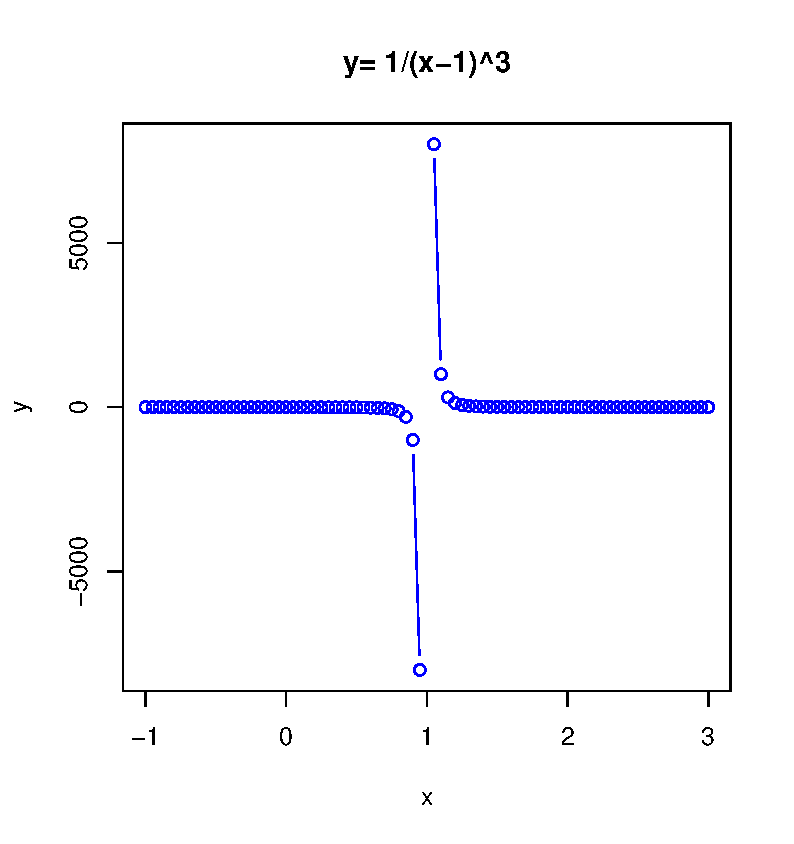
\includegraphics[width=\linewidth]{Plot2a.pdf}
		\phantomsubcaption
		\label{F2a}
	\end{subfigure}
	\hfill
	\begin{subfigure}[t]{0.49\textwidth}
		\centering
		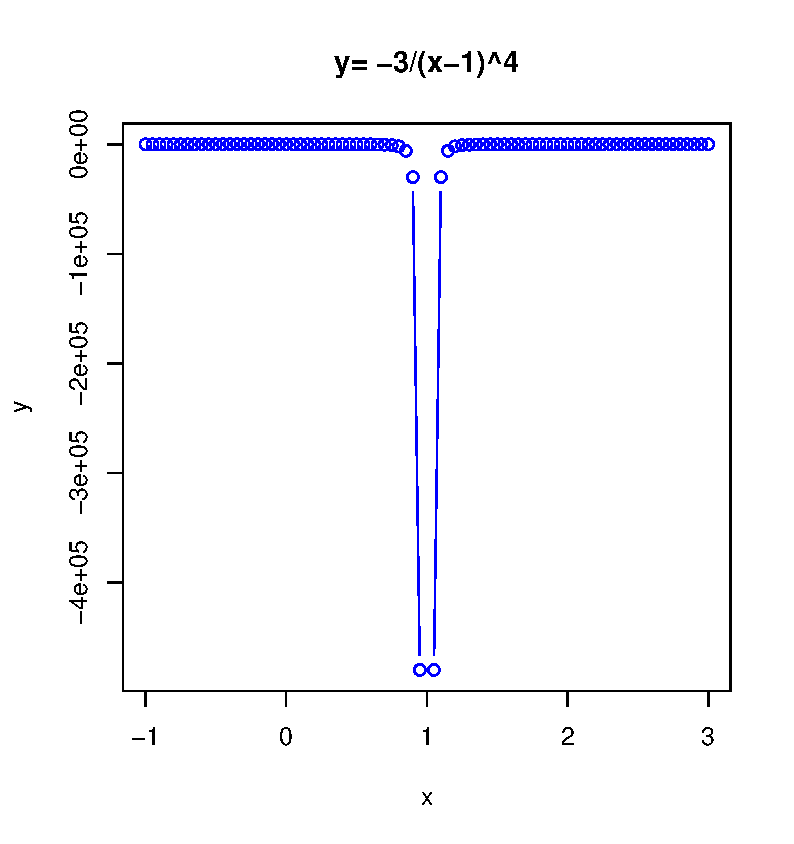
\includegraphics[width=\linewidth]{Plot2b.pdf}
		\phantomsubcaption
		\label{F2b}
	\end{subfigure}
	\caption{(a)Plot of $y=1/(x-1)^3$ generated using R. (b)Plot of $y = -3/(x-1)^4$ generated using R.}\label{F2}
\end{figure}
It's easy to see that the derivative $\mathrm{d}g(x)/\mathrm{d}x = -3/(x-1)^4$ is shown in \autoref{F2b} and does not have a discontinuity at that point, but it can be checked that the integral would be infinite.
Consider the integral $I$ shown below $$I = \int_{0}^{2}\frac{\mathrm{d}x}{(x - 1)^4}$$
Using the direct antiderivate method we get
$$I = \int_{0}^{2}\frac{1}{(x-1)^4}\,\mathrm{d}x = -\frac{1}{3}\frac{1}{(x-1)^3}\bigg\rvert_{0}^{2} = -\frac{2}{3}$$
Now, breaking it up into it constituents as shown below
\begin{align*}
	I &= \int_{0}^{2}\frac{1}{(x-1)^4}\,\mathrm{d}x = \int_{0}^{1^-}\frac{1}{(x-1)^4}\,\mathrm{d}x + \int_{1^+}^{2}\frac{1}{(x-1)^4}\,\mathrm{d}x \\
	&=\frac{1}{3}\frac{1}{(x-1)^3}\bigg\rvert_{1^-}^{0} + \frac{1}{3}\frac{1}{(x-1)^3}\bigg\rvert_{2}^{1^+} \\
	& \to \infty &&
\end{align*}

\section{Second example}

Another example of a discontinuous $g(x)$ is $\tan(x)$ such that $x \in (0, \pi)$.

\begin{figure}[h]
	\centering
	\begin{subfigure}[t]{0.49\textwidth}
		\centering
		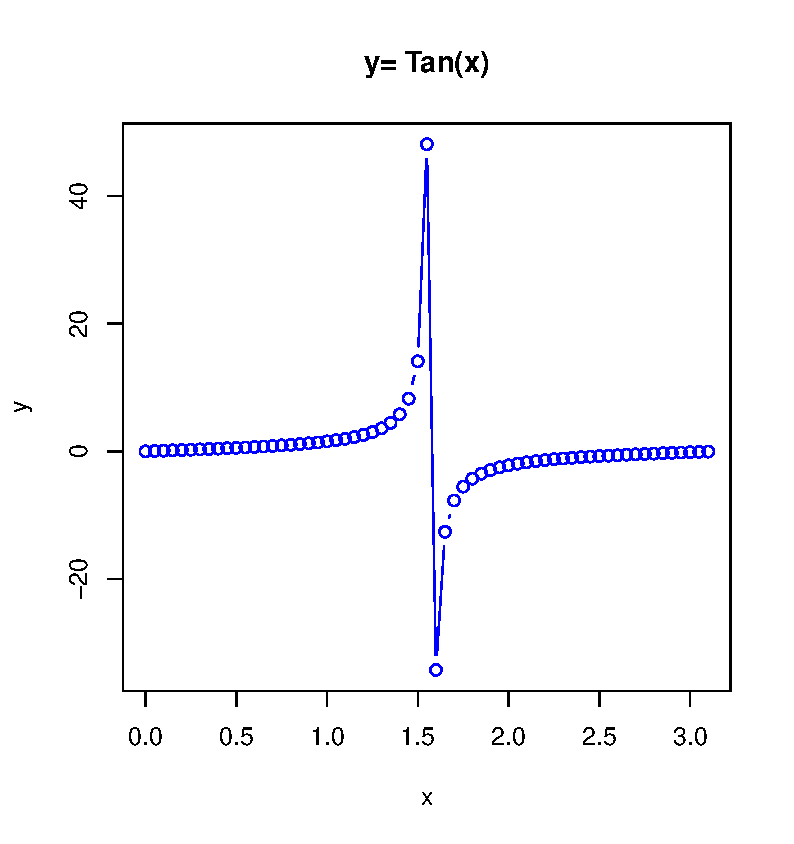
\includegraphics[width=\linewidth]{Plot3a.pdf}
		\phantomsubcaption
		\label{F3a}
	\end{subfigure}
	\hfill
	\begin{subfigure}[t]{0.49\textwidth}
		\centering
		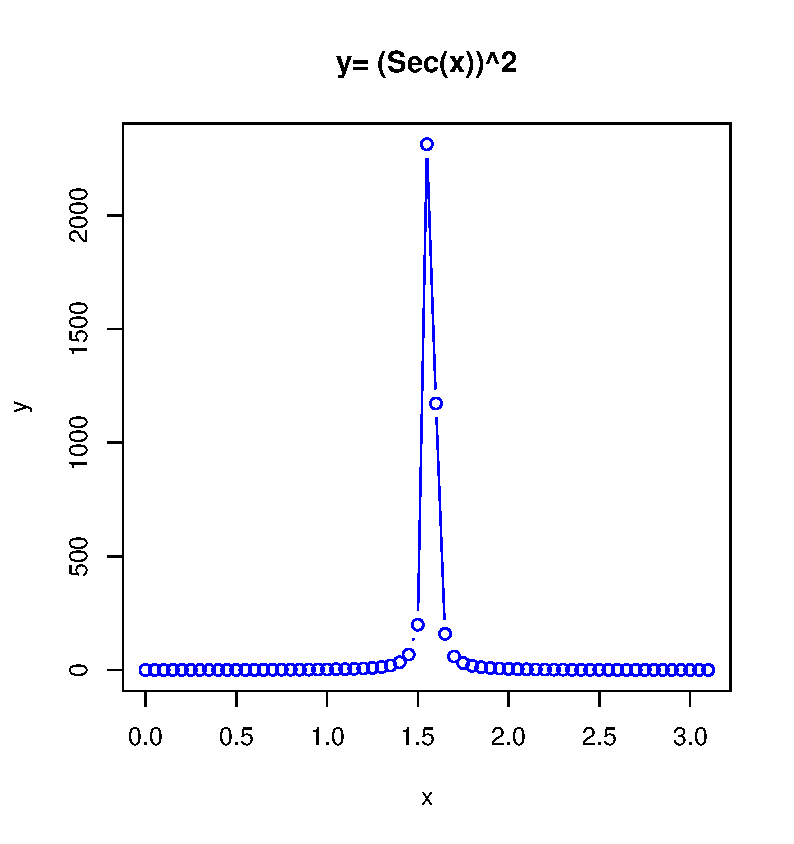
\includegraphics[width=\linewidth]{Plot3b.pdf}
		\phantomsubcaption
		\label{F3b}
	\end{subfigure}
	\caption{(a)Plot of $y=\tan{x}$ generated using R. (b)Plot of $y = (\sec{x})^2$ generated using R.}\label{F3}
\end{figure}

The discontinuity in \autoref{F3a} can be seen at $x =\pi/2$ for $g(x) = \tan{x}$. Thus, the consequence of directly using the antiderivative method for the problem can be seen below and yields a value of zero which is incorrect and can be directly judged from \autoref{F3b}.

\begin{align*}
	I &= \int_{0}^{\pi}\sec^2{x}\,\mathrm{d}x \\
	&= \tan{x}\bigg\rvert_{0}^{\pi} \\
	&= 0
\end{align*}

However, splitting it up into integrals on either side of $\pi/2$ yields the infinitely large area as shown below.

\begin{align*}
	I = \int_{0}^{\pi}\sec^2{x}\,\mathrm{d}x &= \int_{0}^{{\frac{\pi}{2}}^-}\sec^2{x}\,\mathrm{d}x + \int_{{\frac{\pi}{2}}^+}^{\pi}\sec^2{x}\,\mathrm{d}x \\
	&= \tan{x}\bigg\rvert_{0}^{{\frac{\pi}{2}}^-} + \tan{x}\bigg\rvert_{{\frac{\pi}{2}}^+}^{\pi} \\
	& \to \infty
\end{align*}
	\begin{appendices}
		\chapter{Appendix}
\section{Appendix: Code for \autoref{F1a}}
\begin{lstlisting}
	rm(list = ls())
	x <- seq(-1,1, by=0.05)
	y <- 1/x^2
	plot(x,y, col='blue', main = 'y= 1/x^2', type = 'b')
\end{lstlisting}

\section{Appendix: Code for \autoref{F1b}}
\begin{lstlisting}
	rm(list = ls())
	x <- seq(-1,1, by=0.05)
	y <- 1/x
	plot(x,y, col='blue', main = 'y= 1/x', type = 'b')
\end{lstlisting}

\section{Appendix: Code for \autoref{F2a}}
\begin{lstlisting}
	rm(list = ls())
	x <- seq(-1,3, by=0.05)
	y <- 1/(x-1)^3
	plot(x,y, col='blue', main = 'y= 1/(x-1)^3', type = 'b')
\end{lstlisting}

\section{Appendix: Code for \autoref{F2b}}
\begin{lstlisting}
	rm(list = ls())
	x <- seq(-1,3, by=0.05)
	y <- -3/(x-1)^4
	plot(x,y, col='blue', main = 'y= -3/(x-1)^4', type = 'b')
\end{lstlisting}

\section{Appendix: Code for \autoref{F3a}}
\begin{lstlisting}
	rm(list = ls())
	x <- seq(0,pi, by=0.05)
	y <- tan(x)
	plot(x,y, col='blue', main = 'y= Tan(x)', type = 'b')
\end{lstlisting}

\section{Appendix: Code for \autoref{F3b}}
\begin{lstlisting}
	rm(list = ls())
	x <- seq(0,pi, by=0.05)
	y <- 1/(cos(x))^2
	plot(x,y, col='blue', main = 'y= (Sec(x))^2', type = 'b')
\end{lstlisting}
	\end{appendices}
\end{document}